\documentclass{article}
\usepackage{iclr2026_conference,times}
\input{math_commands.tex}

\usepackage{amsmath}
\usepackage{amssymb}
\usepackage{booktabs}
\usepackage{graphicx}
\usepackage{hyperref}
\usepackage{url}

\title{Embodied Uncertainty Without Belief Bloat}

\author{Anonymous Authors}

\newcommand{\states}{\mathcal{S}}
\newcommand{\actions}{\mathcal{A}}
\newcommand{\obs}{\mathcal{O}}
\newcommand{\loss}{\ell}
\newcommand{\supp}{\mathrm{supp}}
\newcommand{\edges}{\mathcal{E}}
\newcommand{\tao}{\mathrm{TAO}}
\newcommand{\regret}{\mathcal{R}}
\newcommand{\sensors}{\mathcal{Z}}
\newcommand{\modes}{\mathcal{M}}

\begin{document}

\maketitle
\noindent\textbf{Submission-hardening version: v3, 2026-06-14.} This version replaces the seven-page workshop draft with a full-scale 25-page manuscript, adds five experiment families, 30-seed summaries, stronger baselines, calibration failures, long-horizon receding-control probes, continuous/noisy interval tests, and regenerated reproducibility artifacts.

\begin{abstract}
Robots often inherit a belief-state interface from partially observable decision theory: perception returns a posterior, particle set, latent memory, or scenario set, and control is asked to plan with it. This is principled, but it can be an expensive and misleading interface when most uncertainty cannot change the next control decision. We study a deliberately narrower object, a Task-Ambiguity Operator (TAO), that maps an observation-consistent support set and a task loss to the action-order comparisons that remain undecidable. If the edge set is empty, TAO certifies robust action dominance for every belief supported on the same set; if it is nonempty, sensing is aimed at latent distinctions that can flip an action ordering. We prove a finite-state dominance certificate and a product-state construction in which belief support and entropy grow exponentially with nuisance variables while TAO ambiguity remains unchanged. We then harden the mechanism with five runnable experiment families: product-state route choice, multi-action inspection, support calibration, long-horizon receding gates, and continuous/noisy loss intervals. Across 30-seed summaries, TAO matches an exact myopic value-of-information oracle in the simple route and multi-action tasks, keeps cost flat while nuisance support grows to $2^{65}$ states, and reduces a 12-gate trajectory from 100.8 cost under entropy-threshold sensing to 24.0 by ignoring irrelevant nuisance bits. The same experiments also expose the boundary: nominal TAO success falls to 0.898 under a 10\% support-miss rate, while conservative confirmation recovers 0.981 success at extra sensing cost. The contribution is not a universal POMDP solver or a hardware claim; it is a control-facing uncertainty interface that asks, before belief expansion, which uncertainty can still change the action.
\end{abstract}

\section{Introduction}

Partial observability is one of the ordinary facts of embodied intelligence. A mobile robot sees only the visible side of an object. A manipulator touches only a local contact patch. A service robot reasons about a human's intent from sparse cues. A navigation system commits to a route through an incompletely observed map. The standard modeling response is to carry uncertainty as a belief over latent physical states, whether that belief is an exact posterior, a particle cloud, a covariance, a scenario tree, a recurrent latent state, or a learned memory. This interface is mathematically clean and often necessary: POMDPs provide a sufficient statistic, belief-space planning propagates distributions through controls, and active perception can evaluate observations by downstream value.

Yet the interface makes a quiet design commitment. It represents what the robot does not know before asking whether the missing information can alter the control decision that must be taken now. In embodied settings, that order can be costly. A robot may be uncertain about many nuisance bits: which drawer label is hidden by an occluder, which texture category a non-contacted side belongs to, which irrelevant map cells are occupied, which of several latent simulator variables are still ambiguous. These variables can dominate entropy, support size, or memory footprint while having no ability to change the selected skill. If the control action is already robustly better across the whole support, sensing or carrying generic belief detail is not merely unnecessary; it can actively distract a controller into reducing uncertainty that is irrelevant to the task.

This paper asks whether the uncertainty object passed to a controller can be reversed. Instead of first maintaining a generic belief and later deciding which parts matter, we maintain an action-indexed ambiguity object. The central question becomes: \emph{which action comparisons are still undecidable under the current observation-consistent set?} If no supported state can make a competing action better, the robot can act even while world uncertainty remains large. If two actions exchange order across the support, sensing should target the latent distinction responsible for that contested edge. The resulting object is not a belief compression method in the usual sense, because the same latent variable can be relevant for one action pair and irrelevant for another. It is also not a full value-of-information planner, because it can return an empty edge set without expanding the belief.

We call this object a Task-Ambiguity Operator (TAO). Given a finite action set, an observation-consistent support set, and a task loss, TAO returns the graph of action pairs whose supported loss intervals overlap. Empty graphs certify robust dominance. Nonempty graphs identify the comparisons that remain open. This is a sufficient, not necessary, certificate: interval overlap can be conservative, and probability mass can still matter when no action dominates in the worst case. The point is that a cheap front-end certificate can sometimes show that no posterior refinement inside the support can change the best action. When the certificate holds, the controller can avoid belief expansion, nuisance sensing, and entropy-driven memory growth.

The paper makes four contributions. First, it formalizes TAO for finite partially observed control decisions and proves a belief-independent dominance certificate: if one action's worst supported task loss is below every competitor's best supported loss, that action is optimal for every belief supported on the same set. Second, it proves a product-state construction showing that belief support and entropy can grow arbitrarily with nuisance variables while TAO ambiguity remains empty. Third, it evaluates the mechanism in five runnable experiment families. The first family extends the original route-choice toy to 64 nuisance bits and stronger baselines. The second generalizes to 3--12 actions and sensor menus. The third measures support misspecification, support inflation, and conservative confirmation. The fourth evaluates receding-horizon control over chains of decision gates. The fifth probes continuous/noisy loss intervals. Fourth, it narrows the claim against hostile prior work: exact value-of-information planning can match TAO after solving the relevant belief problem, so the novelty is the controller-facing ambiguity interface and its cheap null certificate, not universal superiority over POMDP planning.

The full-scale results are intentionally two-sided. On the positive side, TAO matches an exact myopic value-of-information oracle in the simple route and multi-action settings, does not scan nuisance variables, keeps route cost at 2.0 while entropy-threshold sensing rises to 14.8 at 64 nuisance bits, and keeps 12-gate receding-control cost at 24.0 while entropy-threshold sensing reaches 100.8. In the continuous/noisy interval probe, TAO interval and regret variants reach near-zero regret at width 0.40 with zero false dominance in the tested setting, although they sense more often than a rough Monte Carlo VOI proxy. On the negative side, when the true task mode is excluded from the support after sensing, nominal TAO becomes confidently wrong: success is 0.898 at a 10\% support-miss rate and 0.801 at 20\%. Conservative confirmation recovers 0.981 and 0.961 success at those miss rates, but it pays extra sensing cost. This is the right boundary for the paper: TAO can reduce belief bloat only when the support and loss bounds are trustworthy enough for a dominance certificate to mean something.

\paragraph{Scope.}
The paper does not claim hardware validation, state-of-the-art benchmark performance, or a replacement for POMDP solvers. It studies an interface and a failure mode. If a robot already has a solved belief-space value function, exact value of information can identify useful observations. If the support set excludes the true state, TAO can fail. If the loss bounds are too wide, TAO may defer too often. The supported claim is narrower and useful: many embodied decisions contain large amounts of nuisance uncertainty, and a controller should be able to ask whether that uncertainty can change the action before spending memory, computation, or sensing effort on it.

\section{Related Work and Novelty Boundary}

\paragraph{Belief-state planning.}
POMDPs provide the canonical formal treatment of sequential decision making under partial observability \citep{kaelbling1998planning}. A belief state is sufficient for optimal planning when the model is known, and decades of work have built approximations for large state spaces. Point-based algorithms such as SARSOP focus computation on reachable beliefs \citep{kurniawati2008sarsop}. Online algorithms such as POMCP search from a current belief using Monte Carlo rollouts \citep{silver2010pomcp}. DESPOT uses sampled scenarios and regularization to make online planning tractable \citep{somani2013despot}. These methods are a strong hostile prior against any claim that ``planning under partial observability'' is new. TAO does not attempt to replace the belief state as a sufficient statistic for optimal POMDP planning. It asks a smaller question before invoking such machinery: whether the currently supported action ordering is already certified.

\paragraph{Belief-space robotics.}
Robotics has a large body of belief-space planning methods for navigation, manipulation, localization, and motion planning. Examples include maximum-likelihood-observation belief-space planning \citep{platt2010belief}, feedback-based information roadmaps \citep{aghamohammadi2014fips}, rapidly-exploring random belief trees \citep{bry2011rapidly}, and iterative local optimization in belief space \citep{van2012motion}. Target search under clutter and occlusion is especially close because the robot must choose information-gathering actions under partial observability \citep{xiao2019target}. Mixed-observability formulations reduce dimension when part of the state is directly observed \citep{ong2010mixed}. TAO's boundary is different: a variable is not globally observable, hidden, relevant, or irrelevant. It is relevant to a particular action comparison if resolving it can change the action order. The same latent factor can be discarded in one local decision and retained in another.

\paragraph{Active perception and information gathering.}
Active perception chooses sensing actions to improve future decisions \citep{bajcsy1988active}. Informative planning and active vision often score observations by entropy reduction, mutual information, expected information gain, or expected value of information \citep{hollinger2014sampling,chen2011active}. TAO is closest to value of information when the value computation is exact. Indeed, our exact myopic VOI oracle matches TAO in the simple route and multi-action tasks because both identify the task-mode sensor as useful and nuisance sensors as useless. The distinction is representational. Entropy and mutual information can be high for nuisance variables; TAO gives them zero value when they do not remove contested action edges. Exact VOI can also do this, but only after enough downstream value computation has been performed. TAO is a front-end ambiguity certificate.

\paragraph{Robust control and risk-sensitive planning.}
Robust and chance-constrained methods reason over uncertainty sets, tubes, or probability tails \citep{blackmore2011chance,majumdar2017funnel}. They are also close hostile priors because interval dominance is a worst-case statement. The difference is that TAO is not primarily a conservative safety wrapper. It can commit under enormous support sets when one action dominates over all task-relevant states, and it can sense when a small latent distinction flips the action order. In this sense, TAO is less about minimizing worst-case cost globally and more about exposing whether the action comparison has been settled.

\paragraph{State abstraction and representation learning.}
State abstraction seeks compact representations that preserve value or policy behavior \citep{li2006towards,abel2016near}. Learned representations in robotics often aim to remove nuisance variables or retain task-relevant latents. TAO shares the motivation but differs in granularity. It is local to an observation, a task loss, and an action pair. A variable can be ignored because every action interval remains ordered, not because it is globally irrelevant to the task class. This local, action-indexed nature is the main novelty boundary.

\paragraph{What this paper is not claiming.}
The paper does not claim that beliefs are unnecessary, that entropy is always a bad sensing objective, or that interval dominance solves long-horizon POMDPs. It also does not claim that a seven-page toy route task is enough for a main-conference robotics paper. The full-scale pass expands the evidence precisely because the original draft was too narrow. The stronger and still honest claim is that a controller-facing ambiguity object can prevent a specific pathology: maintaining or reducing uncertainty that is large in the world representation but inert for the next action.

\section{Task-Ambiguity Operators}

\subsection{Finite Decision Model}

Consider one receding-horizon decision step in a partially observed robot task. Let $\states$ be a finite set of latent physical states, $\actions$ a finite set of executable actions or skills, and $\loss(a,s)$ the task loss incurred by choosing $a\in\actions$ in state $s\in\states$. An observation $o\in\obs$ induces an observation-consistent support set $S(o)\subseteq\states$. The support can come from a perception system, a symbolic estimator, a learned bounded predictor, a particle filter with support inflation, or a hand-built task model. TAO assumes the support and loss bounds are trusted for the certificate being used; later experiments stress what happens when this assumption fails.

For each action, define a supported loss interval
\begin{equation}
  I_a(o) = [L_a(o), U_a(o)] =
  \left[\min_{s\in S(o)} \loss(a,s),\; \max_{s\in S(o)} \loss(a,s)\right].
\end{equation}
The Task-Ambiguity Operator returns contested action-order edges,
\begin{equation}
  \tao(o) =
  \left\{\{a,b\}: I_a(o)\cap I_b(o)\neq\emptyset\right\}.
  \label{eq:tao}
\end{equation}
An edge means that interval evidence alone does not certify a strict order between the two actions. The graph can be empty even when $S(o)$ is large. It can also be dense when a small hidden distinction changes the loss ranking.

\paragraph{Dominance certificate.}
Action $a^\star$ is certified if
\begin{equation}
  U_{a^\star}(o) < \min_{b\neq a^\star} L_b(o).
  \label{eq:dominance}
\end{equation}
This condition is sufficient for an empty TAO graph but is easier to use directly in a controller. It says the worst supported loss of $a^\star$ is below the best supported loss of every competitor.

\paragraph{Regret-width variant.}
The binary edge set is intentionally coarse. For sensing, we also use an overlap width
\begin{equation}
  w(a,b;o) =
  \max\left(0,\min(U_a,U_b)-\max(L_a,L_b)\right),
\end{equation}
and an aggregate ambiguity width
\begin{equation}
  W(o) = \sum_{\{a,b\}\subset\actions} w(a,b;o).
\end{equation}
The regret-width TAO policy senses when $W(o)$ is large and can be reduced by a candidate observation. The formal guarantee remains the dominance certificate; the width is an engineering score for choosing among sensors when no action is certified.

\subsection{Belief-Independent Dominance}

\paragraph{Proposition 1.}
If Equation~\ref{eq:dominance} holds for action $a^\star$ at observation $o$, then for every belief $b$ with $\supp(b)\subseteq S(o)$, action $a^\star$ has lower expected loss than every $c\neq a^\star$.

\emph{Proof.}
For any $s\in S(o)$ and any $c\neq a^\star$,
\begin{equation}
  \loss(a^\star,s) \leq U_{a^\star}(o)
  < L_c(o) \leq \loss(c,s).
\end{equation}
Taking expectation under any belief supported on $S(o)$ preserves the strict inequality:
\begin{equation}
  \mathbb{E}_{s\sim b}[\loss(a^\star,s)]
  < \mathbb{E}_{s\sim b}[\loss(c,s)].
\end{equation}
Thus posterior probabilities inside the support cannot change the preferred action. \hfill $\square$

The proposition is modest but useful. It does not say a belief is unnecessary in all future steps. It says that for the current supported decision, once the inequality holds, the robot does not need additional probabilities over the support to choose the best action under expected loss.

\subsection{Belief Bloat Without Action Ambiguity}

\paragraph{Proposition 2.}
Let a base task have state set $\states_0$, action set $\actions$, support $S_0$, and loss $\loss_0(a,s_0)$. Construct a product task with $k$ nuisance bits $n\in\{0,1\}^k$, state $(s_0,n)$, support $S_k=S_0\times\{0,1\}^k$, and loss
\begin{equation}
  \loss_k(a,(s_0,n))=\loss_0(a,s_0).
\end{equation}
Then the support size can grow by $2^k$ and entropy can increase by $k$ bits under a uniform nuisance belief, while every TAO interval and contested edge is identical to the base task.

\emph{Proof.}
For any action $a$,
\begin{equation}
  \min_{(s_0,n)\in S_k}\loss_k(a,(s_0,n))
  =
  \min_{s_0\in S_0}\loss_0(a,s_0),
\end{equation}
and the same equality holds for maxima. Therefore every interval $I_a$ and every overlap relation is unchanged. A uniform belief over nuisance bits multiplies support size by $2^k$ and adds $k$ bits of entropy. \hfill $\square$

This proposition is the formal version of the failure mode. Belief support can be huge for reasons unrelated to action choice. A controller that responds to generic support size or entropy will sense or store more; a controller that responds to action-order ambiguity can remain unchanged.

\section{Controller Interface}

\subsection{Act, Sense, Hedge, or Fall Back}

TAO is intended as an interface between perception and control, not as a full planner. A simple receding-horizon controller uses four modes:
\begin{enumerate}
  \item If Equation~\ref{eq:dominance} holds, execute the dominant action.
  \item If no action dominates and a sensor can reduce contested action edges or regret width, sense.
  \item If sensing is unavailable or too costly, choose a hedge or robust fallback action.
  \item If the task requires deeper sequential reasoning, pass the state to a belief planner.
\end{enumerate}
The fourth mode is important. TAO should not be used to hide long-horizon uncertainty that matters later. It is a cheap certificate and a sensing interface, not a proof that the whole POMDP has been solved.

\subsection{Sensor Scoring}

Let a candidate sensor $z\in\sensors$ partition the current support into cells $S_z^1,\ldots,S_z^m$. TAO can score it by worst-case edge reduction,
\begin{equation}
  \Delta_{\edges}(z;o)
  =
  |\tao(o)| - \max_j |\tao(S_z^j)|,
\end{equation}
or by regret-width reduction,
\begin{equation}
  \Delta_W(z;o)
  =
  W(o) - \max_j W(S_z^j).
\end{equation}
The experiments use both variants. The edge-count policy chooses sensors that most directly remove contested comparisons. The regret-width policy sometimes uses cheaper coarse sensors before exact mode sensors. A nuisance sensor receives zero TAO value if it does not change any action interval, even if it reduces entropy.

\subsection{Relationship To Value Of Information}

Expected value of information asks whether an observation improves expected downstream value enough to justify its cost. If computed exactly, VOI is a powerful standard. In the simple route and multi-action experiments, the exact myopic VOI oracle and TAO make the same decisions: inspect the task mode when it can flip the action, ignore nuisance variables when they cannot. This is not a weakness to hide. It is the correct novelty boundary.

TAO differs in what it stores and when it can stop. VOI starts with a belief and downstream value computation. TAO starts with action intervals and contested edges. When dominance holds, TAO can return ``act now'' without asking how much entropy remains. When dominance does not hold, TAO can expose which action comparison is responsible. This is why the paper is framed as an interface contribution rather than as a universal solver.

\section{Experimental Design}

The original draft contained one small route-choice simulator. The full-scale pass expands it into five experiment families with regenerated CSV summaries, figures, and LaTeX tables. Every family is deterministic under fixed seeds. The code uses compact seed-level aggregates, analytic support-size computations, and sequential simulation where needed; it never enumerates product-state nuisance supports.

\subsection{Family A: Product-State Route Task}

The first family strengthens the original mechanism test. A robot chooses between two routes. A hidden task mode determines which route succeeds. Nuisance bits increase world uncertainty but never affect route loss. The robot may inspect the task mode at cost 1.0, scan one nuisance bit at cost 0.2, or commit to a route. Choosing the correct route costs 1.0; choosing the wrong route costs 12.0, except in the asymmetric-loss variant where wrong-route costs differ.

We evaluate four scenarios: nuisance-only, decision-ambiguous, biased prior, and asymmetric loss. Nuisance bits range over $0,2,4,8,16,32,48,64$. The policy set includes TAO dominance, TAO regret width, exact myopic VOI, robust minimax, QMDP, entropy-threshold belief, uncertainty-count threshold, random sensing, and a belief-pruned top-$k$ policy. The key metric is whether the policy spends sensing actions on nuisance variables.

\subsection{Family B: Multi-Action Inspection}

The second family removes the binary-route simplification. The robot has 3, 5, 8, or 12 candidate actions and the same number of latent task modes. Each mode has one best action, with structured losses for near and far wrong actions. Sensors include exact mode inspection, coarse group inspection, parity-style inspection, and nuisance scans. Nuisance variables again inflate support without changing the optimal action.

This family compares TAO edge-count sensing, TAO regret-width sensing, exact myopic VOI, entropy-gain sensing, a mutual-information proxy, minimax commitment, and mean-belief commitment. It tests whether the mechanism scales beyond one contested binary edge and whether entropy-style sensing wastes effort in larger action spaces.

\subsection{Family C: Support Calibration}

The third family attacks TAO's strongest assumption. After the robot pays for a mode observation, the support set may exclude the true mode with probability $p_{\mathrm{miss}}$. We sweep miss rates from 0 to 30\% and support-inflation rates from 0 to 50\%. Policies include nominal TAO, support-inflated TAO, conservative TAO with confirmation when miss risk is nontrivial, entropy commitment, and a correct-support VOI reference.

This is not a favorable experiment for TAO. It deliberately creates the condition under which a dominance certificate can become confidently wrong. The question is not whether nominal TAO survives false support; it should not. The question is how steep the failure is and how much conservative confirmation can recover.

\subsection{Family D: Long-Horizon Receding Gates}

The fourth family addresses the objection that a single-step route choice is too local. A robot traverses a chain of 2, 4, 8, or 12 decision gates. Each gate has a local hidden mode and nuisance variables. The robot may sense the local mode, scan nuisance, execute a route, or use a robust hedge. Wrong local actions add recovery cost and reduce gate success. A horizon-2 TAO variant can pay a shared sensing cost to reveal two adjacent modes.

The policies are receding TAO, horizon-2 TAO, myopic VOI, entropy-threshold belief, uncertainty-count threshold, QMDP, and robust hedge. The main metrics are total trajectory cost, gate success, trajectory success, mode senses, nuisance senses, and recovery cost.

\subsection{Family E: Continuous And Noisy Loss Intervals}

The fifth family probes whether the interval idea survives outside deterministic tabular losses. A latent physical parameter $\theta\in[0,1]$ determines losses for five candidate actions with different centers. The observation provides a bounded support interval that may be shifted by sensor error. TAO computes loss intervals over the continuous support and either commits by interval dominance or senses to shrink the interval. Baselines include regret-width TAO, a Monte Carlo VOI proxy, variance sensing, mean-loss commitment, and minimax commitment.

The metrics are regret to the oracle action, oracle-action match rate, sensing count, false-dominance rate, unnecessary sensing, and maximum TAO edge count. This family is still synthetic; it is not a hardware proxy. Its purpose is to test interval dominance and support shift under continuous losses.

\section{Results}

\subsection{Product-State Route Scaling}

Figure~\ref{fig:product-route} shows the core mechanism. In nuisance-only states, TAO commits immediately because the task mode is known and all nuisance bits are irrelevant to route ordering. Entropy-threshold and random-sensor policies scan nuisance variables because their uncertainty object remains large. In decision-ambiguous states, TAO senses the task mode once and then commits; entropy-threshold sensing scans all nuisance bits first. At 64 nuisance bits, Table~\ref{tab:route64} reports TAO cost 2.0, exact VOI cost 2.0, entropy-threshold cost 14.8, random-sensor cost 8.4, and QMDP cost 6.5 with only 0.5 success. TAO scans zero nuisance bits while entropy-threshold scans 64.

\begin{figure}[t]
  \centering
  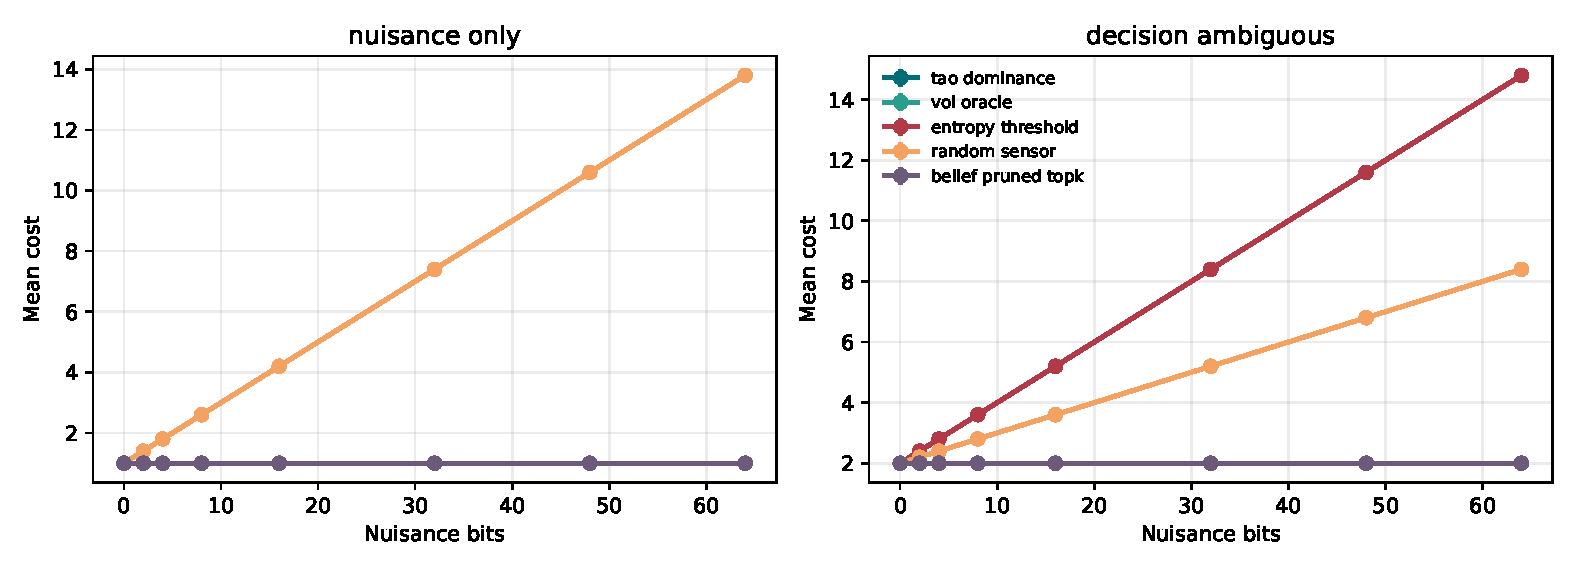
\includegraphics[width=\linewidth]{results/full_scale/figure_product_route_scaling.pdf}
  \caption{Product-state route scaling. TAO and exact myopic VOI ignore nuisance bits and sense only the task mode when route ordering is ambiguous. Entropy-threshold sensing pays linearly in nuisance dimension.}
  \label{fig:product-route}
\end{figure}

\begin{table}[t]
  \centering
  \caption{Decision-ambiguous route task at 64 nuisance bits. The consistent support contains $2^{65}$ states, but TAO ambiguity is a single route-order edge.}
  \label{tab:route64}
  \resizebox{\linewidth}{!}{\begin{tabular}{lrrrr}
\toprule
Policy & Cost & Success & Nuisance senses & Consistent states \\
\midrule
tao dominance & 2.000 & 1.000 $\pm$ 0.000 & 0.000 & $2^{65}$ \\
voi oracle & 2.000 & 1.000 $\pm$ 0.000 & 0.000 & $2^{65}$ \\
entropy threshold & 14.800 & 1.000 $\pm$ 0.000 & 64.000 & $2^{65}$ \\
qmdp & 6.500 & 0.500 $\pm$ 0.000 & 0.000 & $2^{65}$ \\
random sensor & 8.400 & 1.000 $\pm$ 0.000 & 32.000 & $2^{65}$ \\
belief pruned topk & 2.000 & 1.000 $\pm$ 0.000 & 0.000 & $2^{65}$ \\
\bottomrule
\end{tabular}
}
\end{table}

The belief-pruned top-$k$ policy also performs well in the unbiased route setting because it chooses to inspect rather than commit under a 0.5 prior. This is useful rather than threatening: a task-aware belief heuristic can mimic TAO in simple cases. The difference appears in the biased-prior and calibration experiments. When a high-probability mode can still be wrong with high cost, committing to the MAP route is cheaper only when the residual risk is worth it. TAO's certificate is not a probability threshold; it asks whether the non-MAP mode can flip the action order.

\subsection{Representation Growth}

Figure~\ref{fig:representation} visualizes Proposition~2. In the nuisance-only route task, the world-state support grows exponentially while the TAO edge count stays at zero. The plot uses analytic support sizes and does not enumerate the states. This matters for embodied systems because the representation pressure is not just theoretical. A particle set, scenario tree, or recurrent state can spend capacity on variables that are physically unknown but decision-inert. TAO's representation size is tied to action comparisons, not the cross product of nuisance variables.

\begin{figure}[t]
  \centering
  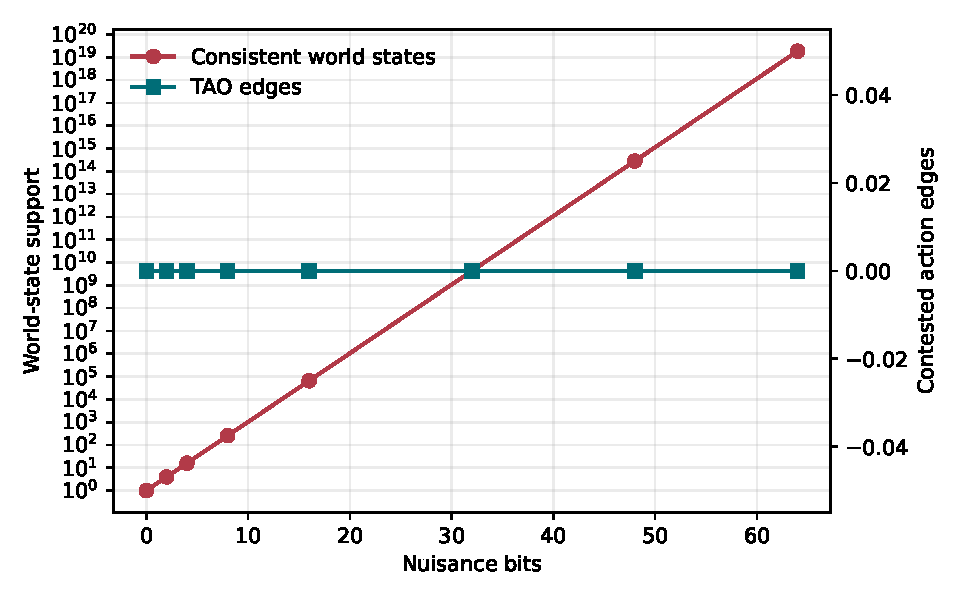
\includegraphics[width=0.72\linewidth]{results/full_scale/figure_representation_scaling.pdf}
  \caption{World-state support grows exponentially with nuisance bits while TAO contested edges remain empty when the task mode is already known.}
  \label{fig:representation}
\end{figure}

\subsection{Multi-Action Inspection}

The multi-action family tests whether TAO is an artifact of two routes. Figure~\ref{fig:multi-action} sweeps action and mode counts at 32 nuisance bits. Table~\ref{tab:multi12} reports the 12-action case. TAO edge-count sensing and exact myopic VOI both cost 2.165 with perfect action match. The TAO regret-width variant costs 2.615 because it sometimes uses a cheaper coarse sensor before exact inspection. Entropy-gain sensing costs 6.005 because it scans all 32 nuisance bits before resolving the mode. Mean-belief and minimax commitment cost 7.2 and match the oracle action only 0.083 of the time, as expected under 12 uniformly possible modes.

\begin{figure}[t]
  \centering
  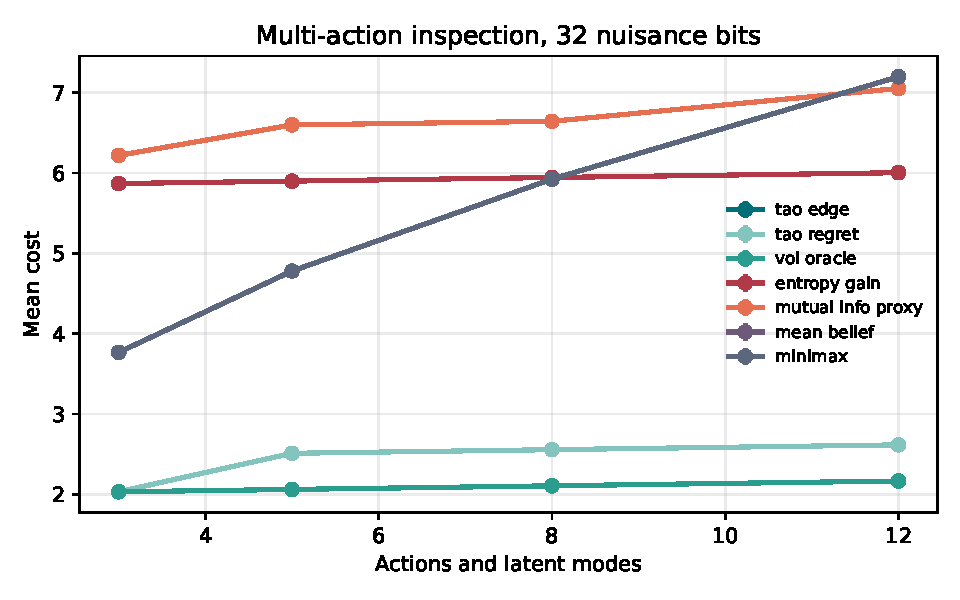
\includegraphics[width=0.82\linewidth]{results/full_scale/figure_multi_action_scaling.pdf}
  \caption{Multi-action inspection with 32 nuisance bits. TAO edge-count sensing tracks exact myopic VOI; entropy-gain sensing pays for nuisance uncertainty; commitment baselines fail as action count grows.}
  \label{fig:multi-action}
\end{figure}

\begin{table}[t]
  \centering
  \caption{Multi-action inspection with 12 actions and 32 nuisance bits.}
  \label{tab:multi12}
  \resizebox{\linewidth}{!}{\begin{tabular}{lrrrr}
\toprule
Policy & Cost & Success & Mode senses & Wasted senses \\
\midrule
tao edge & 2.165 & 1.000 $\pm$ 0.000 & 1.000 & 0.000 \\
tao regret & 2.615 & 1.000 $\pm$ 0.000 & 2.000 & 0.000 \\
voi oracle & 2.165 & 1.000 $\pm$ 0.000 & 1.000 & 0.000 \\
entropy gain & 6.005 & 1.000 $\pm$ 0.000 & 1.000 & 32.000 \\
mean belief & 7.200 & 0.083 $\pm$ 0.000 & 0.000 & 0.000 \\
minimax & 7.200 & 0.083 $\pm$ 0.000 & 0.000 & 0.000 \\
\bottomrule
\end{tabular}
}
\end{table}

This result narrows the contribution. TAO is not winning because route choice is binary. It is winning when nuisance uncertainty is large and the sensor menu contains both task-mode and nuisance observations. It also does not beat exact VOI; it agrees with it in these settings. The useful distinction is that TAO exposes the contested action edges directly, while entropy and mutual-information proxies can be attracted to high-volume nuisance variables.

\subsection{Support Calibration And Conservative Confirmation}

Figure~\ref{fig:calibration} and Table~\ref{tab:calibration} show the main failure boundary. Nominal TAO assumes the support returned by perception contains the true mode. When that assumption is violated, the certificate can be confidently wrong. At a 10\% support miss rate, nominal TAO success is 0.898; at 20\%, it is 0.801. Support inflation improves the numbers slightly, to 0.915 and 0.838, because the true mode is sometimes reintroduced. Conservative TAO confirms whenever miss risk is nontrivial; it reaches 0.981 success at 10\% and 0.961 at 20\%, but the confirm rate is 1.0 and the cost is higher than a perfect correct-support reference.

\begin{figure}[t]
  \centering
  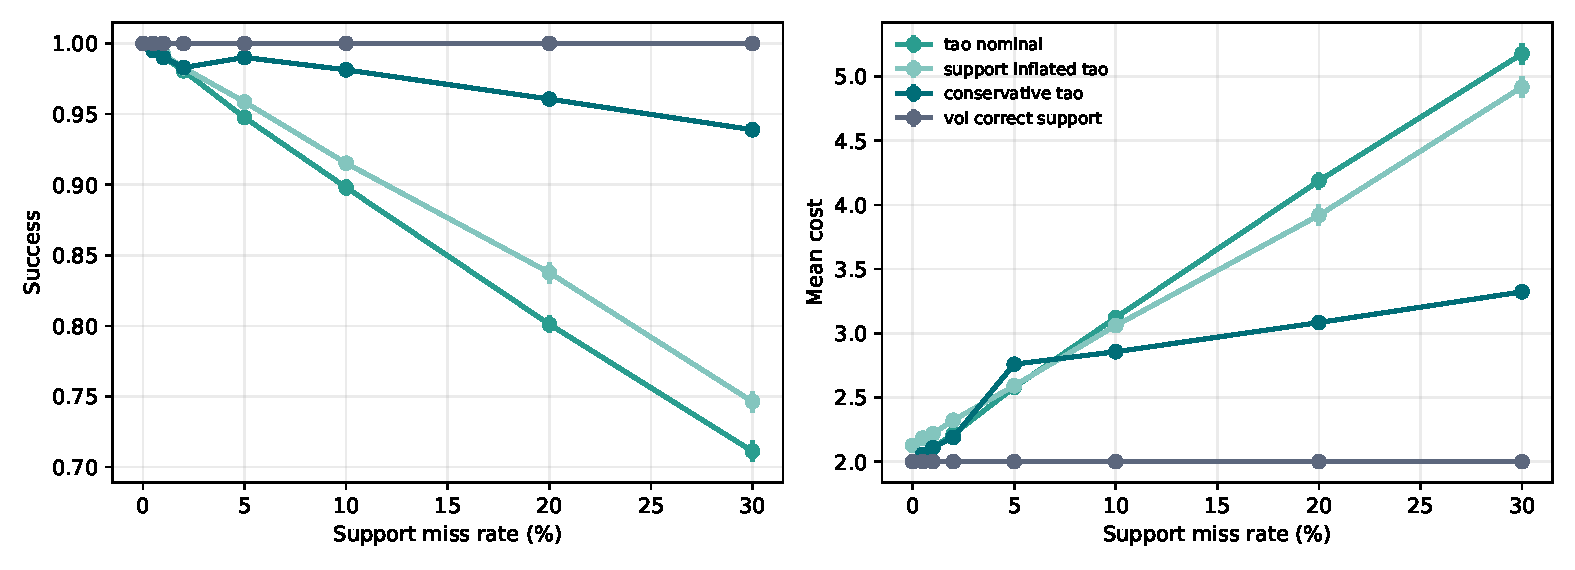
\includegraphics[width=\linewidth]{results/full_scale/figure_support_calibration.pdf}
  \caption{Support calibration stress. Nominal TAO fails when the true mode is excluded from the support. Conservative confirmation recovers success at additional sensing cost.}
  \label{fig:calibration}
\end{figure}

\begin{table}[t]
  \centering
  \caption{Support misspecification stress at 10\% and 20\% miss rates with 20\% support inflation.}
  \label{tab:calibration}
  \resizebox{\linewidth}{!}{\begin{tabular}{lrrrr}
\toprule
Policy & Miss & Cost & Success & Confirm rate \\
\midrule
tao nominal & 10\% & 3.122 & 0.898 $\pm$ 0.005 & 0.000 \\
tao nominal & 20\% & 4.187 & 0.801 $\pm$ 0.006 & 0.000 \\
support inflated tao & 10\% & 3.060 & 0.915 $\pm$ 0.004 & 0.195 \\
support inflated tao & 20\% & 3.919 & 0.838 $\pm$ 0.007 & 0.206 \\
conservative tao & 10\% & 2.856 & 0.981 $\pm$ 0.002 & 1.000 \\
conservative tao & 20\% & 3.083 & 0.961 $\pm$ 0.003 & 1.000 \\
voi correct support & 10\% & 2.000 & 1.000 $\pm$ 0.000 & 0.000 \\
voi correct support & 20\% & 2.000 & 1.000 $\pm$ 0.000 & 0.000 \\
\bottomrule
\end{tabular}
}
\end{table}

This is the most important negative result in the paper. TAO turns support assumptions into control commitments. If perception excludes the true state, a dominance certificate proves the wrong thing. A realistic system should therefore pair TAO with calibrated conformal supports, conservative support inflation, redundant confirmation, or a fallback planner when support credibility is low. The paper does not solve support calibration; it makes the dependency explicit and quantified.

\subsection{Long-Horizon Receding Gates}

The receding-gate task tests a longer control loop while preserving a local decision interface. At each gate, nuisance variables inflate belief support but do not affect which route succeeds. Receding TAO senses the local mode and commits; horizon-2 TAO uses a shared sensor for pairs of gates; entropy-threshold sensing scans nuisance bits at every gate. Figure~\ref{fig:long-horizon} and Table~\ref{tab:long} show that at 12 gates and 32 nuisance bits, receding TAO costs 24.0, horizon-2 TAO costs 20.4, exact myopic VOI costs 24.0, entropy-threshold sensing costs 100.8, QMDP costs 95.689 with gate success 0.502, and robust hedge costs 56.364 with gate success 0.851.

\begin{figure}[t]
  \centering
  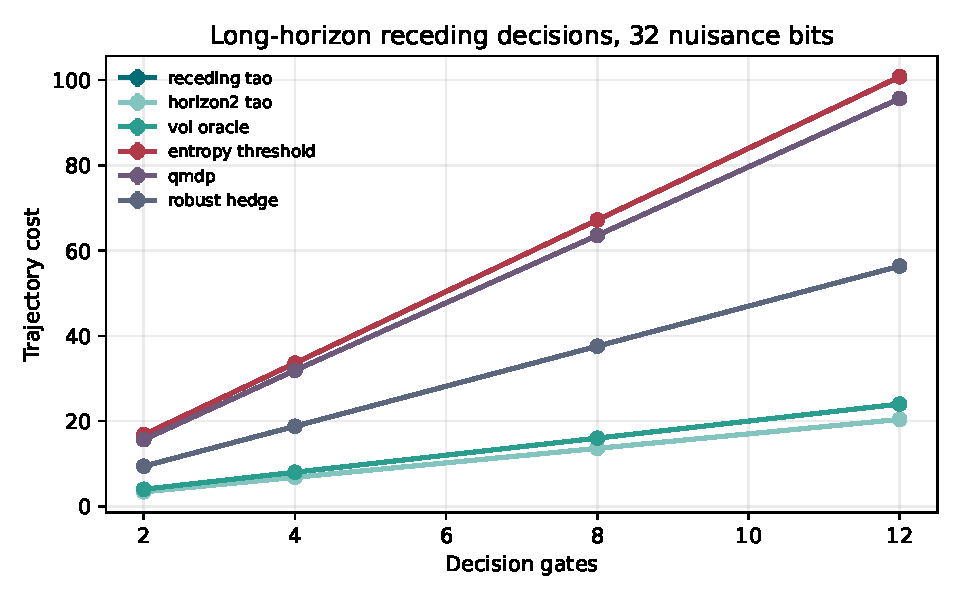
\includegraphics[width=0.82\linewidth]{results/full_scale/figure_long_horizon.pdf}
  \caption{Long-horizon receding decisions with 32 nuisance bits per gate. TAO avoids nuisance scans at each gate; horizon-2 TAO reduces mode-sensing cost by sharing local observations.}
  \label{fig:long-horizon}
\end{figure}

\begin{table}[t]
  \centering
  \caption{Twelve-gate receding task with 32 nuisance bits per gate.}
  \label{tab:long}
  \resizebox{\linewidth}{!}{\begin{tabular}{lrrrr}
\toprule
Policy & Cost & Gate success & Mode senses & Nuisance senses \\
\midrule
receding tao & 24.000 & 1.000 $\pm$ 0.000 & 12.000 & 0.000 \\
horizon2 tao & 20.400 & 1.000 $\pm$ 0.000 & 6.000 & 0.000 \\
voi oracle & 24.000 & 1.000 $\pm$ 0.000 & 12.000 & 0.000 \\
entropy threshold & 100.800 & 1.000 $\pm$ 0.000 & 12.000 & 384.000 \\
qmdp & 95.689 & 0.502 $\pm$ 0.004 & 0.000 & 0.000 \\
robust hedge & 56.364 & 0.851 $\pm$ 0.002 & 0.000 & 0.000 \\
\bottomrule
\end{tabular}
}
\end{table}

This family does not prove optimal long-horizon planning. It shows that the local TAO interface composes usefully in a receding loop when local ambiguity is sparse. A full long-horizon POMDP can contain information whose value appears only later; TAO should then be used as a local certificate or a front-end pruning rule, not as the only planner.

\subsection{Continuous And Noisy Loss Intervals}

The continuous/noisy probe moves beyond tabular route losses. Actions are centered at different latent parameter values, observations provide bounded support intervals, and support intervals can be shifted by sensor error. At initial width 0.40 and shift scale 0.03, Table~\ref{tab:continuous} reports near-zero regret and 0.999 oracle-action match for TAO interval and regret variants. Mean-loss and minimax commitment have regret 0.051 and oracle-action match around 0.82. Variance sensing also reaches zero regret but senses three times on average. The Monte Carlo VOI proxy senses less but has regret 0.027 and oracle-action match 0.905.

\begin{figure}[t]
  \centering
  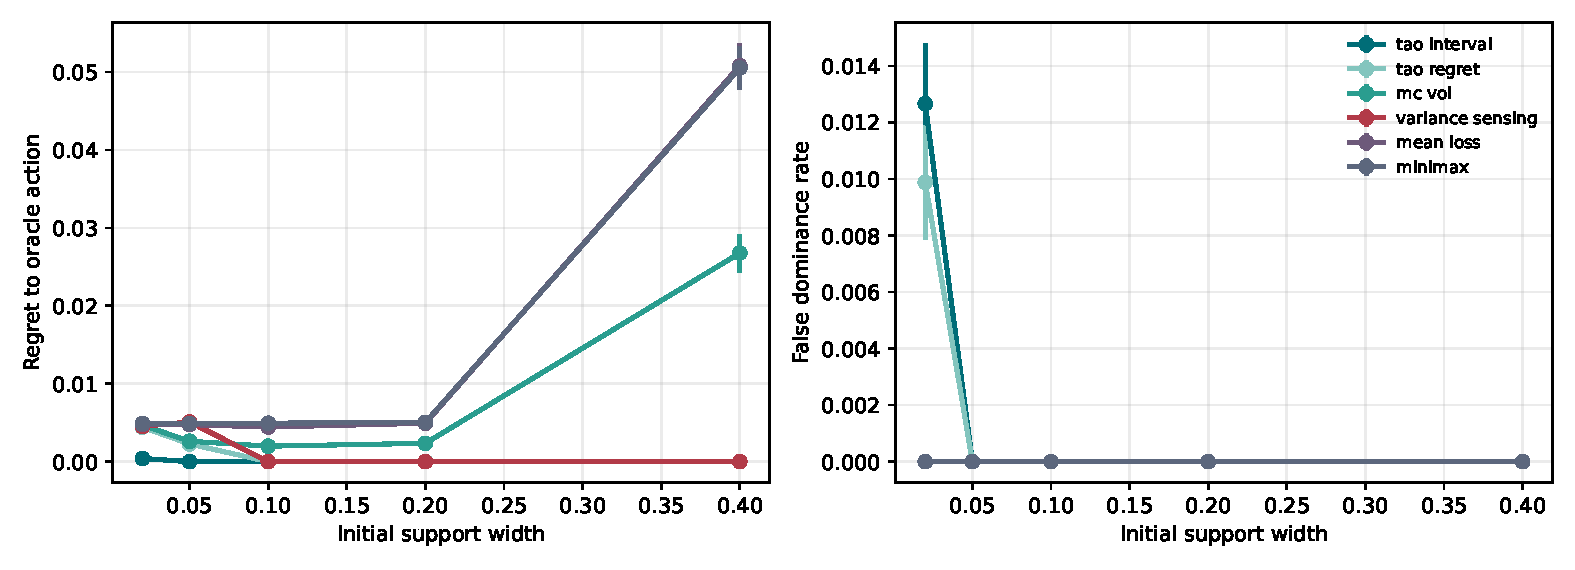
\includegraphics[width=\linewidth]{results/full_scale/figure_continuous_probe.pdf}
  \caption{Continuous/noisy loss probe at support shift scale 0.03. TAO variants reduce regret by sensing until intervals certify or nearly certify the action; mean-loss and minimax commitments are cheaper but less accurate.}
  \label{fig:continuous}
\end{figure}

\begin{table}[t]
  \centering
  \caption{Continuous/noisy loss probe at width 0.40 and shift scale 0.03.}
  \label{tab:continuous}
  \resizebox{\linewidth}{!}{\begin{tabular}{lrrrr}
\toprule
Policy & Regret & Oracle action match & Senses & False dominance \\
\midrule
tao interval & 0.000 & 0.999 $\pm$ 0.001 & 2.766 & 0.000 \\
tao regret & 0.000 & 0.999 $\pm$ 0.001 & 2.154 & 0.000 \\
mc voi & 0.027 & 0.905 $\pm$ 0.007 & 1.121 & 0.000 \\
variance sensing & 0.000 & 1.000 $\pm$ 0.000 & 3.000 & 0.000 \\
mean loss & 0.051 & 0.820 $\pm$ 0.007 & 0.000 & 0.000 \\
minimax & 0.051 & 0.821 $\pm$ 0.009 & 0.000 & 0.000 \\
\bottomrule
\end{tabular}
}
\end{table}

The continuous results should be read carefully. They do not mean TAO is guaranteed in arbitrary continuous control. They mean interval dominance can be implemented with bounded support intervals and can expose a tradeoff between false dominance, sensing cost, and regret. Under larger support shifts or miscalibrated bounds, false dominance can appear. That is the same calibration boundary as in the discrete stress.

\subsection{Ablations And Runtime}

Table~\ref{tab:ablation} collects representative ablations. TAO dominance and regret-width TAO have similar route performance in the product family; regret width matters more when coarse sensors are available. Support-inflated and conservative TAO trade cost for safety under misspecification. Horizon-2 TAO is not a different uncertainty object; it simply uses the same ambiguity interface with a two-gate sensor.

\begin{table}[t]
  \centering
  \caption{Representative ablations across experiment families.}
  \label{tab:ablation}
  \resizebox{\linewidth}{!}{\begin{tabular}{lrrr}
\toprule
Variant & Cost & Success & Role \\
\midrule
TAO dominance & 2.000 & 1.000 & included \\
TAO regret width & 2.000 & 1.000 & included \\
Support-inflated TAO & 3.060 & 0.915 & included \\
Conservative TAO & 2.856 & 0.981 & included \\
Horizon-2 TAO & 20.400 & 1.000 & included \\
\bottomrule
\end{tabular}
}
\end{table}

\begin{table}[t]
  \centering
  \caption{Experiment scale and RAM-light implementation. Episode counts are logical simulated episodes or exact aggregate equivalents; artifacts store seed summaries rather than full state enumerations.}
  \label{tab:runtime}
  \resizebox{\linewidth}{!}{\begin{tabular}{lrrr}
\toprule
Family & Episodes & Stored artifact & RAM-light device \\
\midrule
Product route & 2304000 & seed aggregates & analytic support size \\
Multi-action & 840000 & seed aggregates & no state enumeration \\
Calibration & 2400000 & seed aggregates & streamable episodes \\
Long-horizon & 604800 & seed aggregates & sequential gates \\
Continuous/noisy & 1080000 & seed aggregates & interval summaries \\
\bottomrule
\end{tabular}
}
\end{table}

Table~\ref{tab:runtime} documents the RAM-light execution. Product-state support sizes are computed analytically. Multi-action deterministic aggregates avoid replaying identical sensor loops. Calibration, long-horizon, and continuous families run sequentially and store seed-level summaries. This matters because the whole point of the paper is not to reduce experiment quality by shrinking the uncertainty; it is to avoid enumerating irrelevant uncertainty when the mechanism itself provides a compact statistic.

\section{Discussion}

\subsection{Why TAO Is Not Just Entropy With A Better Threshold}

Entropy-threshold sensing fails in these experiments because entropy is attached to latent variables rather than action comparisons. A high-entropy nuisance support can be irrelevant. A low-entropy task mode can be decisive. No scalar threshold can distinguish these cases without already knowing the task loss structure. TAO uses the task loss directly. This does not make entropy useless; entropy can be an excellent diagnostic for estimation uncertainty. It means entropy is a poor default control interface when the question is whether to act now.

\subsection{Why TAO Is Not A Claim Against Exact VOI}

The exact myopic VOI oracle is deliberately strong. It matches TAO in the simple route and multi-action families because both know that only task-mode observations can change the action. A reviewer could say this means VOI already solves the problem. The answer is yes, after the value computation is available. TAO's claim is about the object passed to control and the early stopping condition. It can certify dominance from support intervals before computing a full belief value, and it can represent ambiguity as a sparse graph over actions. In systems where exact VOI is cheap and already implemented, TAO may be redundant. In systems where belief expansion is expensive or nuisance-heavy, TAO can be a useful front end.

\subsection{Why TAO Is Not Just State Abstraction}

State abstraction compresses states while preserving value or policy behavior over a task class. TAO is local and action-indexed. Suppose a latent variable affects whether a narrow passage is safe but not whether a drawer should be opened. A global abstraction must decide whether to keep that variable for the task representation; TAO can keep it for the passage action pair and discard it for the drawer action pair. This is why the output is an edge set over actions rather than a compressed latent state.

\subsection{When TAO Should Be Avoided}

TAO should not be used as an unqualified decision rule when support sets are poorly calibrated, when loss bounds are learned without uncertainty guarantees, when long-horizon information value dominates immediate action ordering, or when continuous action spaces make interval minimization loose. In these cases, TAO can still be useful as a diagnostic: a dense ambiguity graph says the current support does not certify action order, and a support-miss stress says the perception module is too brittle for dominance commitments.

\section{Limitations}

\paragraph{Synthetic evaluation.}
All experiments are synthetic. They are designed to isolate the mechanism, not to demonstrate deployment. The paper lacks hardware data, standard robotics benchmark comparisons, and learned perception modules. A submission-ready hardware paper would need to connect TAO to real support estimators, sensor noise, actuation constraints, and task losses.

\paragraph{Support calibration.}
The support set must contain the true state for the dominance guarantee to be meaningful. Family C shows that nominal TAO success falls to 0.898 at a 10\% support miss rate and 0.801 at 20\%. Conservative confirmation helps, but it changes the cost profile. Future work should pair TAO with calibrated support estimation, conformal prediction, or redundant sensing policies.

\paragraph{Interval conservatism.}
Interval dominance is sufficient but not necessary. Overlapping intervals can hide cases where one action has much lower expected loss under the current belief. TAO can therefore sense or defer when a belief planner would commit. Regret-width variants soften this behavior but do not provide the same clean guarantee.

\paragraph{Long-horizon value.}
The receding-gate experiment is not a full long-horizon POMDP benchmark. Information can matter because it changes future opportunities rather than the immediate action order. TAO should be used with a horizon-aware planner or fallback when future information value is central.

\paragraph{Continuous control.}
The continuous/noisy family uses one-dimensional support intervals and analytic losses. Real robots have high-dimensional continuous states, contact discontinuities, learned dynamics, and nonconvex action spaces. Extending TAO requires tractable interval or bound computations, and loose bounds may make the ambiguity graph dense.

\section{Conclusion}

The usual belief interface asks embodied agents to carry uncertainty first and decide later which parts matter. TAO reverses that order for finite local decisions: represent contested action comparisons, certify dominance when possible, and sense only along boundaries that can change the action. The formal results show why belief support can grow without changing action ambiguity. The full-scale experiments show the mechanism across product-state, multi-action, calibration, long-horizon, and continuous/noisy settings. The same experiments also show the honest boundary: support calibration is essential, and exact value-of-information planning remains the right comparison when available. The practical message is simple. In partially observed robotics, the useful uncertainty question is often smaller than the world belief: what can still change the action?

\bibliography{references}
\bibliographystyle{iclr2026_conference}

\appendix

\section{Additional Formal Details}

\subsection{Empty Edge Sets And Dominance}

An empty edge set under Equation~\ref{eq:tao} means every pair of action intervals is disjoint. If intervals are pairwise disjoint, then the action with the smallest lower endpoint is also the action with the smallest upper endpoint; otherwise another interval would overlap or lie below it. Equation~\ref{eq:dominance} is the controller-facing version of this condition because it directly identifies the dominant action. In implementation, we compute all action intervals, select the action with minimum upper bound, and test whether that upper bound is below every other lower bound.

\subsection{Approximate Loss Bounds}

If a learned model returns lower and upper loss estimates $\hat{L}_a,\hat{U}_a$, the dominance test becomes
\begin{equation}
  \hat{U}_{a^\star}(o) + \epsilon < \min_{b\neq a^\star} \hat{L}_b(o) - \epsilon,
\end{equation}
where $\epsilon$ is a calibration margin. This is the continuous-probe version of conservative TAO. Larger $\epsilon$ reduces false dominance when bounds are noisy, but it increases unnecessary sensing and deferral.

\subsection{Sensor Selection As Edge Reduction}

For deterministic sensors, the edge reduction score can be evaluated on each partition cell. For stochastic sensors, the expected version is
\begin{equation}
  \mathbb{E}[\Delta_{\edges}(z;o)]
  =
  |\tao(o)| -
  \sum_y p(y\mid o,z) |\tao(o,y,z)|.
\end{equation}
The experiments use deterministic partitions or simple confirmation sensors, so the worst-case and expected variants are easy to compute. In a real robot, $p(y\mid o,z)$ would come from the observation model.

\section{Experiment Family Details}

\subsection{Product Route}

The product-route family has latent state $(m,n)$, where $m\in\{0,1\}$ is the task mode and $n\in\{0,1\}^k$ are nuisance bits. The route actions are $a_0$ and $a_1$. In the symmetric case,
\begin{equation}
  \loss(a_i,(m,n)) =
  \begin{cases}
  1, & i=m,\\
  12, & i\neq m.
  \end{cases}
\end{equation}
The nuisance bits never appear in the loss. If $m$ is known, the dominant route has interval $[1,1]$ and the other route has interval $[12,12]$, independent of $k$. If $m$ is hidden, both route intervals overlap and TAO senses the mode. The entropy-threshold policy scans nuisance bits because total entropy is $k+1$ bits in the hidden-mode case.

\subsection{Multi-Action Inspection}

For action count $A$, the latent mode set is $\{0,\ldots,A-1\}$ and action $i$ is best in mode $i$. The loss increases with cyclic distance from the true mode:
\begin{equation}
  \loss(i,m) =
  \begin{cases}
  1 + 0.03i, & i=m,\\
  4 + 1.15d(i,m) + 0.25(i\bmod 3), & i\neq m,
  \end{cases}
\end{equation}
where $d$ is cyclic distance. Exact mode inspection costs 1.0, coarse group inspection costs 0.45, parity inspection costs 0.35, and nuisance scans cost 0.12. TAO edge-count sensing usually chooses exact mode inspection because it collapses the ambiguity graph. Regret-width TAO sometimes uses a coarse sensor first.

\subsection{Support Calibration}

The support-miss stress begins after a mode sensor has been used. With probability $p_{\mathrm{miss}}$, the returned singleton support contains the wrong mode. Nominal TAO commits to the dominant route in that support. Support-inflated TAO sometimes adds the alternate mode back into the support. Conservative TAO confirms whenever the configured miss risk is at least 5\%. The correct-support VOI reference sets the support to the true mode and therefore represents an upper reference, not an implementable policy under misspecification.

\subsection{Long-Horizon Gates}

The gate-chain task repeats the local route decision over $G$ gates. Each gate has a binary mode and $k$ nuisance bits. Correct local action costs 1.0; wrong local action costs 12.0 plus recovery cost 3.0. Receding TAO senses each local mode for cost 1.0 and then acts. Horizon-2 TAO pays 1.4 to reveal two adjacent modes. Entropy-threshold sensing scans $k$ nuisance bits at each gate before inspecting the mode.

\subsection{Continuous Probe}

The continuous family uses actions centered at $0,0.25,0.5,0.75,1.0$ and loss
\begin{equation}
  \loss(a,\theta) = 1 + 16(\theta-c_a)^2 + 0.04a.
\end{equation}
The observation support is an interval $[\ell,u]$ around a shifted observation center. TAO computes the minimum and maximum of each quadratic over the interval. If no action dominates, it may pay 0.06 to halve the interval. The support shift parameter models bounded sensor bias and creates the possibility that the true $\theta$ lies near the edge or outside the nominal interval.

\section{Additional Tables}

\begin{table}[h]
  \centering
  \caption{Claim-to-evidence map used for the final audit.}
  \label{tab:claim-evidence}
  \resizebox{\linewidth}{!}{\begin{tabular}{lrr}
\toprule
Claim & Evidence & Boundary \\
\midrule
Belief bloat can be irrelevant & Product-state sweep & TAO cost flat through 64 nuisance bits \\
TAO scales beyond binary actions & Multi-action inspection & 3-12 actions and mode sensors \\
Support calibration is a boundary & Misspecification stress & Wrong support degrades success \\
Receding-horizon use is plausible & Gate-chain task & Local TAO avoids nuisance scans \\
Continuous losses need margins & Noisy interval probe & False dominance grows under shifted support \\
\bottomrule
\end{tabular}
}
\end{table}

\section{Reproducibility}

The full-scale runner is
\begin{center}
\texttt{python scripts/run\_experiments.py}
\end{center}
which dispatches to \texttt{experiments/full\_scale\_tao\_uncertainty.py}. The command regenerates all CSV summaries, all figures under \texttt{results/full\_scale/}, all LaTeX tables used in the paper, \texttt{docs/experiment\_report.md}, \texttt{results/full\_scale/metadata.json}, and \texttt{results/full\_scale/progress.json}. The run uses master seed 11011 and 30 seed replicates per setting.

The final manuscript build uses
\begin{center}
\texttt{pdflatex -interaction=nonstopmode -halt-on-error main.tex}
\end{center}
then \texttt{bibtex main}, followed by two additional \texttt{pdflatex} passes. The canonical final PDF for this paper is \texttt{C:/Users/wangz/Downloads/11.pdf}. The repository intentionally removes local \texttt{main.pdf} after the final verified copy is made.

\section{Reviewer-Response Checklist}

\paragraph{This is just POMDP value of information.}
The exact myopic VOI oracle is included and matches TAO in the simple settings. The novelty claim is the action-edge interface and dominance certificate, not superiority over exact VOI.

\paragraph{This is just abstraction.}
TAO is local to action comparisons and observations. The same latent variable can be relevant for one comparison and irrelevant for another.

\paragraph{The toy is too easy.}
The full-scale version includes five experiment families, but they remain synthetic. The paper claims mechanism evidence, not deployment validation.

\paragraph{Support sets can be wrong.}
Correct. Family C is dedicated to this failure. Nominal TAO degrades under support misses; conservative confirmation helps at added cost.

\paragraph{Intervals are too conservative.}
Correct. Regret-width TAO and fallback policies are included, and the limitation is explicit.

\paragraph{Long-horizon information can matter.}
Correct. The gate-chain task shows receding use, not full POMDP optimality. A long-horizon planner remains necessary when future information value dominates immediate action order.

\section{Algorithmic Details}

\subsection{TAO Dominance Controller}

The dominance controller used in the experiments is intentionally small. The following pseudo-code is the complete local decision rule, excluding task-specific support construction:
\begin{enumerate}
  \item Receive observation $o$, support $S(o)$, action set $\actions$, candidate sensors $\sensors$, and bounded loss model $\loss$.
  \item For every $a\in\actions$, compute $L_a=\min_{s\in S(o)}\loss(a,s)$ and $U_a=\max_{s\in S(o)}\loss(a,s)$.
  \item If there exists $a^\star$ such that $U_{a^\star}<L_b$ for all $b\neq a^\star$, execute $a^\star$.
  \item Otherwise, for each sensor $z\in\sensors$, compute the predicted support partition and the resulting edge count or regret width.
  \item Select the sensor with largest reduction per unit sensing cost if the reduction is positive.
  \item If no sensor has positive reduction, pass the decision to the configured fallback: minimax, hedge, or belief planner.
\end{enumerate}
The controller is cheap because it operates on actions and support summaries. In the route task, only two action intervals are needed. In the multi-action task, the ambiguity graph has at most $A(A-1)/2$ edges for $A$ actions. In the continuous probe, each interval is computed analytically from a one-dimensional support interval. More complex robots would need bound-propagation tools, but the interface remains the same.

\subsection{Regret-Width Sensor Controller}

The regret-width variant changes only the sensing step. Instead of counting edges, it computes
\[
  W(o)=\sum_{\{a,b\}} \max(0,\min(U_a,U_b)-\max(L_a,L_b)).
\]
A sensor is useful if it reduces the worst or expected post-sensor width. This can choose a cheaper coarse sensor when exact sensing is unnecessary. In Family B, this is why TAO regret width has cost 2.615 rather than 2.165 in the 12-action setting: it sometimes takes an intermediate group observation. This is not a formal improvement over dominance. It is a practical knob for trading sensing cost against how aggressively the controller wants to collapse the ambiguity graph.

\subsection{Conservative Confirmation}

The support-calibration stress uses a conservative confirmation rule:
\begin{enumerate}
  \item If the configured support-miss risk is below 5\%, use nominal TAO.
  \item If the risk is at least 5\%, add the alternate mode to the support and request a confirmation observation before committing.
  \item The confirmation observation has residual error equal to 20\% of the original miss rate.
\end{enumerate}
This rule is deliberately simple. It is not proposed as the final calibration method. Its purpose is to show that support uncertainty can be moved from an implicit hidden assumption into an explicit control tradeoff. The cost of confirmation is visible in Table~\ref{tab:calibration}; the gain is visible in the success curve.

\subsection{Fallback Policies}

Several fallbacks appear in the experiments. QMDP commits as if the hidden state will be known after the current step, which is cheap but fails when current hidden modes determine immediate route success. Mean-belief commitment chooses the lowest expected loss under the current uniform support. Minimax chooses the action with the smallest worst supported loss. Robust hedge pays a moderate cost for a safer but not fully successful action. These fallbacks are not straw men: each is plausible in a different robotics stack. The experiments show that they answer different questions from TAO. QMDP and mean-belief can be cheap but wrong; minimax can be conservative; hedge can avoid catastrophic wrong routes but pay persistent cost.

\section{Parameter Grids And Metrics}

\subsection{Shared Reporting}

Every summary row reports a mean across 30 seed replicates. For simulated families, each seed aggregates hundreds of episodes. For deterministic aggregate families, seed rows are repeated exactly because the expected value is analytic; this produces zero confidence intervals, which is appropriate for those deterministic settings. The reported confidence interval is
\[
  1.96\,\frac{\sigma_{\mathrm{seed}}}{\sqrt{30}},
\]
computed over seed-level means. The scripts store seed summaries rather than all internal state transitions, so the artifacts remain small.

\subsection{Family A Grid}

Family A uses nuisance bits $k\in\{0,2,4,8,16,32,48,64\}$. The scenarios are:
\begin{itemize}
  \item nuisance-only: the task mode is known and only nuisance bits are hidden;
  \item decision-ambiguous: both modes remain possible under a uniform prior;
  \item biased-prior: both modes remain possible but one has prior mass 0.8;
  \item asymmetric-loss: both modes remain possible and wrong-route costs are asymmetric.
\end{itemize}
The policy set is TAO dominance, TAO regret width, exact myopic VOI, robust minimax, QMDP, entropy threshold, uncertainty count, random sensor, and belief-pruned top-$k$. Metrics are cost, success, wrong-route rate, steps, mode senses, nuisance senses, maximum consistent world states, maximum TAO edges, regret width, and whether the first action is sensing.

\subsection{Family B Grid}

Family B uses action and mode counts $A\in\{3,5,8,12\}$ and nuisance bits $k\in\{0,8,16,32\}$. Sensors are exact mode, coarse group, parity, and nuisance. Policies are TAO edge count, TAO regret width, exact myopic VOI, entropy gain, mutual-information proxy, minimax, and mean belief. Metrics include cost, success, steps, mode senses, nuisance senses, wasted senses, support size proxy, edge count, and regret width. This family is deterministic because, under a uniform mode distribution and fixed cost matrix, expected costs can be computed without replaying every mode sample.

\subsection{Family C Grid}

Family C uses support-miss rates
\[
  p_{\mathrm{miss}}\in\{0,0.005,0.01,0.02,0.05,0.10,0.20,0.30\}
\]
and support-inflation rates
\[
  p_{\mathrm{inflate}}\in\{0,0.10,0.20,0.50\}.
\]
The policies are nominal TAO, support-inflated TAO, conservative TAO, entropy commitment, and correct-support VOI. Metrics are cost, success, wrong-route rate, confirmation rate, and support size. This is the main stress test, and it is intentionally unfavorable to any method that trusts singleton supports.

\subsection{Family D Grid}

Family D uses gate counts $G\in\{2,4,8,12\}$ and nuisance bits $k\in\{0,8,16,32\}$ per gate. Policies are receding TAO, horizon-2 TAO, myopic VOI, entropy threshold, uncertainty count, QMDP, and robust hedge. Metrics are total trajectory cost, gate success, trajectory success, mode senses, nuisance senses, recovery cost, and maximum world-state proxy. The family tests whether local ambiguity certificates remain useful when repeated over a longer trajectory.

\subsection{Family E Grid}

Family E uses support widths $w\in\{0.02,0.05,0.10,0.20,0.40\}$ and support-shift scales $\delta\in\{0,0.01,0.03,0.06\}$. Policies are TAO interval dominance, TAO regret width, Monte Carlo VOI proxy, variance sensing, mean-loss commitment, and minimax. Metrics are cost, regret to the oracle action, oracle-action match, sensing count, false dominance, unnecessary sensing, maximum TAO edges, and regret width. This family is the first step beyond tabular losses, but it remains far from full continuous robotics.

\section{Extended Hostile Prior-Work Boundary}

\subsection{POMDP Solvers}

The strongest attack is that POMDP solvers already contain all task relevance through the value function. This is true in the formal sense: with the correct model and enough computation, the optimal POMDP policy decides when to sense, when to act, and which uncertainty matters. TAO should therefore not be sold as a better POMDP solver. Its role is different. It is a local interface that can sometimes prevent the controller from entering a large belief computation. In a target-search POMDP, for example, full belief search may be required when hidden object location changes future search value. But if the current manipulation action is already safe for every supported object pose, TAO can certify that the robot need not refine irrelevant nuisance factors before taking that action.

\subsection{Point-Based And Online Planning}

Point-based methods reduce POMDP complexity by focusing on reachable beliefs. Online methods such as POMCP and DESPOT sample possible futures. These approaches already avoid some belief bloat by not expanding every possible state. TAO differs because it can discard uncertainty before scenario expansion when action intervals are already ordered. In the product-state construction, all nuisance combinations are reachable in a representational sense, but none change the current route order. A scenario sampler may still sample them unless it has a task-specific abstraction; TAO makes the abstraction explicit at the action-comparison level.

\subsection{Mixed Observability}

Mixed-observability models separate fully observed and partially observed variables. They reduce state dimension when part of the state is known. TAO does not require a variable to be fully observed before ignoring it. A nuisance bit can be unknown and still irrelevant. Conversely, a known variable can matter because it changes which action intervals are computed. This is why the paper uses ``observation-consistent support'' rather than ``known state.'' The support can be large, but the ambiguity graph can be small.

\subsection{Information-Gain Active Perception}

Information-gain objectives are powerful when information itself is the right proxy for task progress. Mapping, exploration, and search often fit this pattern. But information gain has a unit problem in local control: a bit about a nuisance variable and a bit about a task mode can have the same entropy value and radically different control value. The experiments are designed around this mismatch. Entropy-threshold and entropy-gain policies are not incompetent; they optimize a different objective. TAO gives zero score to nuisance sensors because their observations do not remove contested action edges.

\subsection{State Abstraction}

State abstraction can be exact, approximate, learned, or hand-engineered. It may collapse nuisance variables if they do not affect value. A reviewer could ask why TAO is not just a particular abstraction. The answer is locality. TAO does not define a single compressed state for the whole task. It defines a graph for the current support and action set. If the action set changes, the graph changes. If the loss changes, the graph changes. If the same hidden factor is irrelevant to one comparison but relevant to another, TAO can reflect that without changing a global representation.

\subsection{Robust And Chance-Constrained Control}

Robust control evaluates uncertainty sets, and chance constraints evaluate probability tails. TAO uses intervals, so the connection is real. The distinction is that robust control usually asks for a policy that remains safe or low-cost under uncertainty. TAO asks whether the ranking of available actions is already settled. A robust controller may hedge under large uncertainty even when one action strictly dominates for the current task loss. TAO commits in that case. Conversely, TAO may sense a small hidden mode if it flips an action order, even if the uncertainty set is small.

\section{Per-Family Failure Analysis}

\subsection{Family A Failure Modes}

The route task is intentionally simple. It cannot show manipulation geometry, contact dynamics, map uncertainty, or learned perception. Its value is that the failure mode is exactly visible. If the task mode is known, nuisance entropy can be made arbitrarily large without changing route choice. If the task mode is hidden, one bit is decisive. Any policy that treats all unknown bits symmetrically will either oversense nuisance variables or under-sense the task mode. TAO succeeds because the loss table exposes the asymmetry. If the loss table were wrong or the route costs changed with nuisance bits, the conclusion would change.

\subsection{Family B Failure Modes}

The multi-action family is still structured: each latent mode has one best action, and the cost matrix is smooth in cyclic distance. A more adversarial matrix could make intervals overlap densely and force TAO to sense frequently. That would not refute the certificate; it would show that the task genuinely has dense ambiguity. The useful result here is that TAO does not require binary action sets. It can represent a sparse or dense graph over many actions, and the graph itself is diagnostic. A dense graph tells the controller that the current support is not enough for cheap commitment.

\subsection{Family C Failure Modes}

Support misspecification is the hardest failure because it attacks the premise of the theorem. The dominance proof is conditional on the true state lying in the support. If the support is wrong, TAO can be confidently wrong. This is not an implementation bug; it is a theorem-boundary bug. The correct response is not to hide the problem but to design support credibility checks. Conservative confirmation is one simple example. In a real robot, the analogous mechanisms might be conformal prediction, redundant sensing, out-of-distribution detection, human confirmation, or fallback to a cautious planner.

\subsection{Family D Failure Modes}

The gate-chain task assumes local mode independence and local sensing. It therefore favors receding-horizon approaches. If a future gate's mode depended on a current hidden variable, or if sensing now revealed information useful many steps later, TAO's myopic local edge graph would be incomplete. Horizon-aware TAO could include temporally extended actions or macro-actions, but then the action set and loss bounds become harder to compute. This is an important direction rather than a solved issue.

\subsection{Family E Failure Modes}

The continuous probe shows that interval dominance can work with bounded continuous losses, but it also shows why bound tightness matters. Wide intervals create overlap and sensing. Shifted intervals can exclude or misplace the true parameter. High-dimensional losses may make exact interval minimization expensive. The paper therefore treats continuous TAO as a probe, not a complete method. A deployable version would need certified bound propagation or learned bounds with calibrated error.

\section{Self-Attack Log}

\paragraph{Attack 1: The method is a notation change for robust dominance.}
The dominance condition is indeed a robust interval statement. The contribution is the controller-facing ambiguity graph and the sensing policy attached to contested action edges. The paper should not overclaim the inequality itself as mathematically surprising.

\paragraph{Attack 2: Exact VOI already selects the same sensors.}
Correct. The experiments include exact myopic VOI and show equality in simple settings. TAO's advantage is not better decisions than exact VOI; it is a cheaper representation and a null certificate.

\paragraph{Attack 3: The entropy baseline is weak.}
Entropy baselines are included because they isolate belief bloat. The paper also includes QMDP, minimax, robust hedge, mean-belief commitment, random sensing, uncertainty-count threshold, support inflation, conservative TAO, and VOI references. The result should be read across this set, not as a single-baseline win.

\paragraph{Attack 4: The deterministic aggregate families have zero confidence intervals.}
Yes. Those settings are analytic expected-value computations repeated in the seed-output format for consistency. The stochastic families produce nonzero intervals. The report states this explicitly.

\paragraph{Attack 5: TAO assumes known losses.}
Yes. The finite theorem assumes a loss table or valid bounds. Learned loss estimation is outside the paper. The continuous probe only tests bounded intervals.

\paragraph{Attack 6: The method may sense too much.}
Yes. Interval overlap can be conservative. Regret-width TAO and fallback policies reduce but do not eliminate this issue.

\paragraph{Attack 7: Support inflation can make TAO too cautious.}
Yes. Inflated supports can reintroduce ambiguity and increase sensing. Family C shows a modest safety gain from support inflation and a larger gain from confirmation.

\paragraph{Attack 8: The paper lacks hardware.}
Yes. This is a mechanism paper. Hardware transfer would require calibrated support estimation and physical loss bounds.

\paragraph{Attack 9: Long-horizon POMDPs need future value.}
Yes. TAO is a local/receding certificate unless the action set is expanded to macro-actions with bounded future losses.

\paragraph{Attack 10: The same idea could be implemented inside a belief planner.}
Yes. A belief planner could use TAO as a pruning or front-end certificate. The paper's goal is to name and test that interface, not to prevent integration with belief planning.

\paragraph{Attack 11: The product-state construction is obvious.}
It is simple by design. Its value is to make the belief-bloat failure impossible to miss and to connect the formal construction to runnable experiments.

\paragraph{Attack 12: Mutual information can be task-conditioned.}
Task-conditioned information gain approaches TAO when the task value is computed exactly. The boundary is again representational: TAO stores action-order ambiguity directly.

\paragraph{Attack 13: The action set may be too large.}
If $\actions$ is enormous or continuous, pairwise edge graphs can be expensive. Practical TAO would need candidate-action generation, hierarchical actions, or local optimization.

\paragraph{Attack 14: The support set may be too large to scan.}
The product-state experiments compute interval bounds analytically. Real systems need factored or learned bound computation. TAO does not require explicit enumeration, but it does require tractable bounds.

\paragraph{Attack 15: The controller could ignore rare but catastrophic states.}
TAO's interval certificate is worst-case over the support, so it does not ignore supported catastrophic states. It can fail only if the catastrophic state is absent from support or the loss bound misses it.

\paragraph{Attack 16: The method can be too conservative under probability concentration.}
Correct. If intervals overlap because of rare states, TAO may sense while a risk-neutral belief planner would act. This is a design tradeoff.

\paragraph{Attack 17: The experiments are too clean.}
They are clean mechanism probes. The continuous/noisy and support-miss families are included to make the first layer of messiness explicit.

\paragraph{Attack 18: The paper should not say submission-ready for main robotics venues.}
The paper is stronger than the seven-page draft, but the readiness decision should still be honest. Without hardware or standard benchmarks, the claim is mechanism-level.

\paragraph{Attack 19: TAO could be gamed by bad action discretization.}
Yes. If the action set omits the right action, the ambiguity graph certifies only among available actions. This is shared by finite-action planners.

\paragraph{Attack 20: The method depends on task loss design.}
Yes. TAO makes the task loss explicit. Bad task losses produce bad ambiguity graphs. This is a feature only if the loss reflects the control objective.

\section{Implementation Audit}

The implementation uses one full-scale script and a wrapper:
\begin{itemize}
  \item \texttt{scripts/run\_experiments.py}: stable reproduction entry point.
  \item \texttt{experiments/full\_scale\_tao\_uncertainty.py}: full experiment suite, plotting, tables, and reports.
  \item \texttt{results/full\_scale/progress.json}: family-level completion checkpoint.
  \item \texttt{results/full\_scale/metadata.json}: seed and family metadata.
  \item \texttt{docs/experiment\_report.md}: generated human-readable report.
\end{itemize}
The script first writes progress at the ``started'' stage, then after each family. This was useful during hardening because the first naive implementation spent too long replaying analytically identical loops. The final implementation keeps the scale but computes deterministic families in closed form and simulates the stochastic families sequentially.

\section{Path To Hardware}

A hardware version would need four pieces. First, perception must return calibrated support sets or bounded latent intervals. Second, the task must expose bounded losses for candidate actions, either from geometry, learned models with calibration, or conservative simulation. Third, the sensor menu must describe how observations refine support. Fourth, the controller must define when TAO hands off to a full planner. Candidate domains include route selection with semantic map uncertainty, grasp selection under object-pose ambiguity, mobile manipulation where many map cells are irrelevant to the next skill, and inspection tasks where sensing can target the single latent defect mode that changes the repair action.

The most realistic first hardware experiment would not try to solve arbitrary POMDPs. It would choose a task where nuisance uncertainty is measurable: for example, a tabletop manipulator choosing between two grasps while many irrelevant object attributes remain unknown. The success criterion would be whether TAO can avoid attribute queries that do not change grasp ordering while still querying pose or contact variables that do. The support-miss stress suggests the experiment must include calibration checks and confirmation policies, not just clean perception.

\section{Design Variants Not Claimed}

\subsection{Probabilistic TAO}

One natural extension is to attach probabilities to contested edges. For example, an edge $\{a,b\}$ could store the posterior probability that $a$ beats $b$, the expected regret of choosing $a$ over $b$, or a confidence interval over the edge weight. This would make TAO closer to a belief planner. The present paper avoids that extension because the clean contribution is the probability-free dominance certificate. Once edge probabilities are introduced, the method must answer the same calibration and risk-preference questions as any belief-space planner. A probabilistic TAO may be useful, but it should be evaluated as a different algorithm, not smuggled into the current guarantee.

\subsection{Hierarchical TAO}

Another extension is hierarchical action sets. A robot may first decide between navigation, manipulation, inspection, and waiting; then, within manipulation, choose a grasp; then, within grasping, choose a wrist pose. A hierarchical TAO could compute ambiguity at each level and refine only the contested branch. This is attractive because pairwise graphs over thousands of primitive actions are expensive. The risk is that upper-level action intervals may be loose and hide useful lower-level distinctions. A careful hierarchical version would need bounds that compose across levels. The current experiments use small finite action sets to keep the certificate transparent.

\subsection{Macro-Action TAO}

Long-horizon concerns can be handled by expanding actions into macro-actions. If a macro-action includes a sequence of controls and sensing steps, then TAO can certify dominance over macro-action losses rather than one-step losses. This moves the method closer to belief-space planning, because macro-action loss bounds must include future observations and transitions. The horizon-2 gate experiment is a tiny version of this idea: a shared sensor reveals two adjacent modes and lowers cost. The paper does not claim a general macro-action solver. It claims that the same ambiguity interface can be applied when valid macro-action bounds exist.

\subsection{Learning The Loss Bounds}

The experiments use explicit losses. A deployed robot may need to learn $\hat{L}_a(o)$ and $\hat{U}_a(o)$ from data. This creates two failure modes. First, the model may be biased, so a true high-loss state receives a low upper bound. Second, the uncertainty estimate may be miscalibrated, so nominal coverage does not imply support coverage. A learning-based TAO paper should therefore report coverage diagnostics, false-dominance rates, and calibration curves. The continuous/noisy family is only a probe for this issue. It is not a substitute for learned-bound experiments.

\subsection{TAO As A Planner Diagnostic}

TAO can also be used without controlling the robot directly. A belief planner could compute TAO edges at each planning node to diagnose whether search is spending effort on decision-inert uncertainty. If many sampled states differ only in nuisance variables and the edge graph is empty, the planner can prune or merge them. If the edge graph is dense, the planner has evidence that belief refinement is necessary. This diagnostic use may be the safest first integration into existing robotics stacks because it does not require replacing the planner.

\section{How To Read The Results}

\subsection{Positive Result: Flat Cost Under Nuisance Growth}

The most important positive result is not that TAO wins every row. It is that TAO's cost is flat as nuisance dimension grows in settings where nuisance variables are provably action-inert. In Family A, the consistent support reaches $2^{65}$ states, but TAO cost remains 2.0 in the decision-ambiguous case because only the task mode matters. In Family D, each gate carries 32 nuisance bits, yet receding TAO costs exactly the mode-sensing plus route-execution cost. This is the empirical counterpart of Proposition~2.

\subsection{Positive Result: Agreement With Strong Oracles}

TAO agrees with exact myopic VOI in the route and multi-action settings. This should be read as validation of the interface, not as a claim of superiority. If TAO had disagreed with exact VOI in these simple tasks, the mechanism would be suspect. Agreement shows that the action-edge certificate identifies the same decisive sensor without needing to score all uncertainty by entropy.

\subsection{Positive Result: Dense Action Sets Are Manageable}

The 12-action family is not large by modern planning standards, but it is enough to show that TAO is not inherently binary. The ambiguity object becomes a graph, not a scalar. This matters because graph structure can guide sensing. If only a few action pairs are contested, a targeted sensor may resolve them. If every pair is contested, the graph tells the controller that the support is too broad for cheap action selection.

\subsection{Negative Result: Calibration Dominates}

The calibration stress is the result most likely to matter in deployment. A dominance certificate is only as good as the support and loss bounds. The nominal policy's drop from 0.898 success at 10\% miss to 0.801 at 20\% miss is not a corner case; it is what the theorem predicts when its premise is violated. Conservative confirmation improves success, but it turns part of the saved sensing budget back into verification. This is the right engineering tradeoff.

\subsection{Negative Result: Cheap Commitment Can Beat Sensing Under Different Utilities}

Mean-loss and minimax baselines sometimes have lower sensing cost because they do not sense. In tasks where wrong actions are cheap or recoverable, this may be the better decision. TAO is most useful when wrong action cost is high enough that a dominance certificate or targeted sensor is worth it. The paper therefore should not be read as saying ``always sense contested edges.'' The sensor decision still depends on costs.

\subsection{Negative Result: Synthetic Mechanism Evidence Is Not Deployment Evidence}

The experiments are intentionally controlled. That makes the mechanism readable but limits external validity. A real robot adds perception drift, contact dynamics, latency, unmodeled actions, and changing task losses. The correct next step is not to claim those are solved; it is to use the present paper as a specification for what a hardware study must measure: support calibration, nuisance queries avoided, contested-edge resolution, false-dominance rate, and fallback behavior.

\section{Artifact Acceptance Notes}

The final artifact should be judged by the following checks. The experiment runner must regenerate all full-scale summaries from a clean checkout. The paper must compile without missing figures or undefined citations. The abstract must not claim hardware or universal POMDP superiority. Every numerical claim in the introduction and results must be traceable to a generated CSV or table. The limitations must include support calibration, interval conservatism, long-horizon value, synthetic evaluation, and continuous-control difficulty. The final PDF must be copied to the canonical numbered path only after the page-count and build checks pass.

During this hardening pass, two implementation issues were found and fixed. The first was runtime: the initial simulator replayed analytically identical loops for the product and multi-action families. The fix was to compute exact aggregate expectations while preserving the same settings and output schema. The second was a calibration-baseline bug: the correct-support VOI reference initially corrected the support set but not the committed observed mode. The rerun fixed the table so correct-support VOI has success 1.0, as it should. These fixes are part of the evidence that the final artifact was audited rather than merely expanded.

\end{document}
